\newpage
\section{Cel projektu}
Celem projektu jest stworzenie aplikacji pozwalającej na uzyskanie i zwizualizowanie danych dotyczących obecnego członkostwa danego kraju w sojuszu militarnym, a typami posiadanych przez niego gąsienicowych wozów bojowych (czołgów).\\
\indent Zrealizowany projekt jest odpowiedzią na brak możliwości uzyskania tego rodzaju zestawu danych w prosty i szybki sposób. Zebrane w ten sposób informacje mogą dostarczać materiał do interesujących analiz z pogranicza dziedzin takich jak militaria, historia oraz polityka.\\
Link do strony: \url{https://tankify.netlify.com/}\\
Link do repozytorium: \url{https://github.com/moniszcz/TASS}
\begin{figure}[H]
    \centering 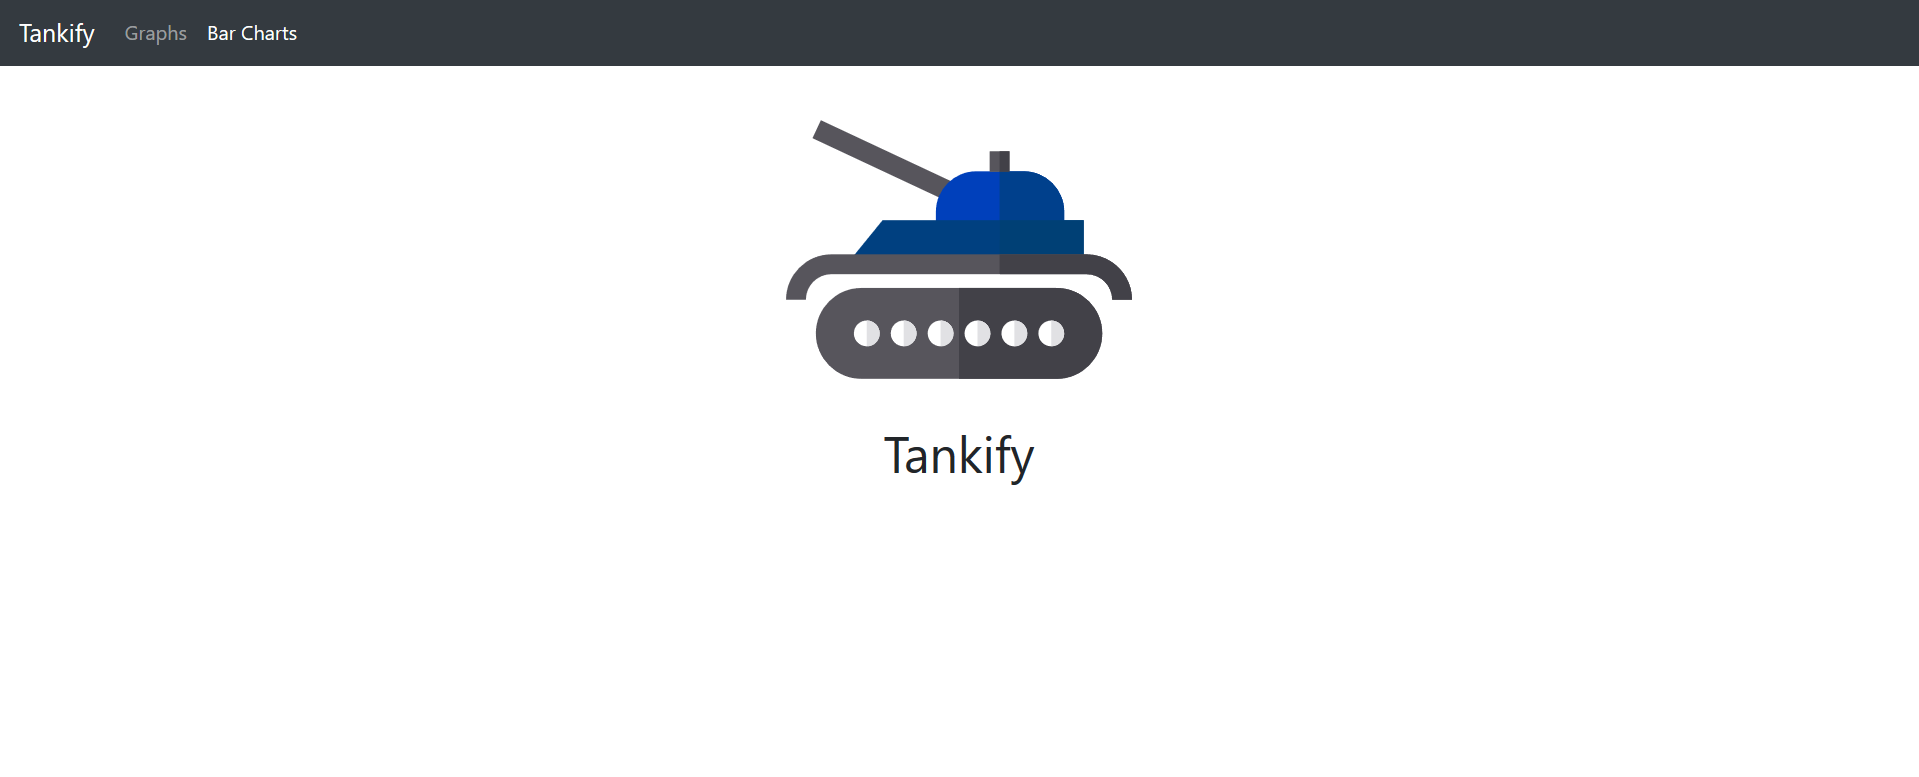
\includegraphics[width=1.0\linewidth]{tex/landing_page.PNG}
    \caption{Strona główna.}
    \label{fig:landing_page}
\end{figure}
\section{Opis aplikacji}
Niezbędne obliczenia na backendzie zostały wykonane przy wykorzystaniu języka programowania \textbf{Python 3.7}, a prezentacja uzyskanych w ten sposób wyników na frotendzie została stworzona przy pomocy technologii \textbf{HTML, CSS, Javascript ES6}. Zebrane dane są przechowywane w bazie danych \textbf{SQLite}, a zapytania są wykonywane przy wykorzystaniu pakietu \textbf{SQL Alchemy}.
\newpage
\subsection{Biblioteki}
Wszystkie wykorzystane biblioteki są zgodne z MPV 2.0 z koncepcji projektu.
 \begin{longtable}{| m{0.2\linewidth} |  m{0.6\linewidth} |} 
     \caption{Biblioteki.} \\ 
     \hline
      \multicolumn{1}{|c|}{Pakiet} & \multicolumn{1}{c|}{Opis} \\ \hline \endfirsthead
    
     \endfoot
     \hline \endlastfoot
    \textit{requests} & wysyłanie zapytań HTTP - pobieranie danych \\ \hline
    \textit{beautifulsoup4} & parsowanie strony HTML/XML \\ \hline
    \textit{NetworkX} & wykonywanie obliczeń grafowych \\ \hline
    \textit{D3js} & wykreślanie grafów \\ \hline   
    \textit{Chart.js} & rysowanie wykresów \\ \hline
    \textit{SQLAlchemy} & mapowanie obiektowo-relacyjne \\ \hline
    \textit{React} & interfejs graficzny aplikacji \\ \hline
    \textit{Flask} & stworzenie endpointów dla GUI\\ \hline
\end{longtable}

\subsection{Technika wykonania}
\subsubsection{Dane}
Niezbędne dane dotyczące posiadanych przez kraje czołgów zostały pobrane, a następnie dostosowane do potrzeb projektu ze strony\cite{dcp19} przy wykorzystaniu techniki webscrapingu oraz pakietów requests oraz beautifulsoup4. \\
Informacje na oryginalnej stronie były zawarte w tabelach uporządkowanych alfabetycznie względem nazwy kraju. Interesującymi z perspektywy projektu informacjami były te zawarte w kolumnach: \textit{Country, Type, Quantity (Estimated), Origin}. Podczas procesu czyszczenia danych napotkaliśmy na następujące problemy:
\begin{itemize}
    \item ilości czołgów podane wraz ze znakami specjalnymi takimi jak ',' , '+', '–'; informacje uzupełniające podane w nawiasach,
    \item niewystarczająca ilość danych dla części krajów (brak szacowanej liczby pojazdów bojowych, skrótowe dane zawarte w formie jednej kolumny),
    \item brak ciągłości zapisu nazw typów czołgów, na przykład używane zamiennie "MBT-2000" \ oraz "MBT 2000". \\
\end{itemize}
\indent W celu przygotowania danych do analizy, zostały zastosowane wyrażenia regularne na kolumnie \textit{Quantity}.\\
Typy czołgów zostały częściowo zagregowane do bardziej ogólnych nazw, z pominięciem modeli. Ten zabieg został wykonany wyłącznie ze względu na specyfikę projektową, aby móc zaobserwować więcej korelacji pomiędzy poszczególnymi państwami. Agregacja została przeprowadzona ręcznie ze względu na stosunkowo niewielką liczbę wierszy, która finalnie wynosi 280. \\
Państwa, dla których była pominięta liczba czołgów oraz te, które posiadały jedynie skrótowe informacje zostały w procesie webscrapingu pominięte.\\
\indent Informacje o sojuszach między krajami zostały pobrane ze strony\cite{alliance} w formie pliku o nazwie ``alliance\_v4.1\_by\_directed`` z rozszerzeniem .csv. Dane użyteczne z perspektywy tematyki projektu znajdują się w kolumnach \textit{state\_name1, state\_name2, dyad\_st\_year, dyad\_end\_year} i zawierają odpowiednio: pierwsze dwie: nazwy krajów, kolejne lata rozpoczęcia i zakończenia sojuszu. Dane uzyskane z tej strony są spójne. Ze względu na szeroką rozpiętość czasową zawartych w tym zbiorze informacji, do analizy zostały uwzględnione tylko te sojusze, które nie posiadają daty zakończenia. Jest to podyktowane faktem posiadania jedynie bieżących informacji o ilościach uzbrojenia dla konkretnych krajów. Analizowanie danych historycznych w tym kontekście wydaje się pozbawione sensu, ponieważ połączenia między ilościami posiadanych czołgów a przeszłymi sojuszami byłyby niemiarodajne. Jesteśmy świadomi faktu, że jest to metoda podatna na błędy, wynikające chociażby z braku znajomości konkretnej daty zakończenia sojuszu, ale sugerując się wysoką jakością pozostałych pobranych danych, zakładamy, że do realizowanego projektu jest to podejście właściwe.\\
Finalna ilość wierszy, po przygotowaniu danych, wynosi 1568.
Nazwy krajów zostały zunifikowane dla obu tabel, zmiany zostały wprowadzone w niewielu przypadkach, na przykład ``Republic of Congo"\ zostało zastąpione  ``Congo".

\subsubsection{Baza danych}
Ze względu na stosunkowo niedużą ilość indywidualnych danych została wykorzystana baza danych SQLite.\\
Baza danych będzie składać się z trzech, połączonych kluczami obcymi, tabel \textit{Tank, Country, Alliance}.
Relacyjny model bazy danych nie uległ zmianom w stosunku do formy przedstawionej w koncepcji wykonania projektu.
\begin{figure}[H]
    \centering 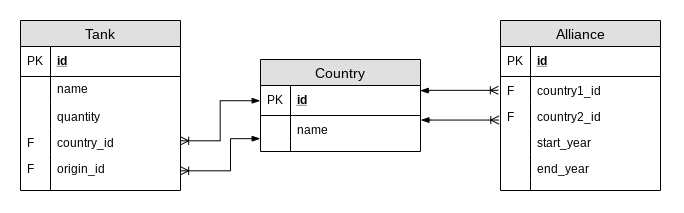
\includegraphics[width=0.8\linewidth]{tex/relacyjna_baza_danych.png}
    \caption{Relacyjny model baza danych.}
    \label{fig:rel_model}
\end{figure}
Tabela \textit{Tank} posiada dwa obowiązkowe klucze obce do tabeli \textit{Country}, odnoszące się do kraju posiadającego dany czołg, oraz do państwa, w którym został wyprodukowany dany pojazd.
Tabela \textit{Alliance} posiada dwa klucze obce do tabeli \textit{Country} będące odniesieniami do krajów, które są w sojuszu. 
\subsection{Scenariusze użycia aplikacji}
\subsection{Wykres krajów posiadających ten sam typ wozu bojowego}
Pierwszym scenariuszem użycia aplikacji jest stworzenie wykresu słupkowego przedstawiającego ilości posiadanych danego typu czołgów przez państwa. Użytkownik ma możliwość wyboru typu uzbrojenia z listy, oraz wpisania minimalnego progu ilościowego. Pozwala to między innymi na ``odsianie`` krajów mających w swoich zasobach jednostkowe ilości czołgów i zawężenie obszaru analizy.
\begin{figure}[H]
    \centering 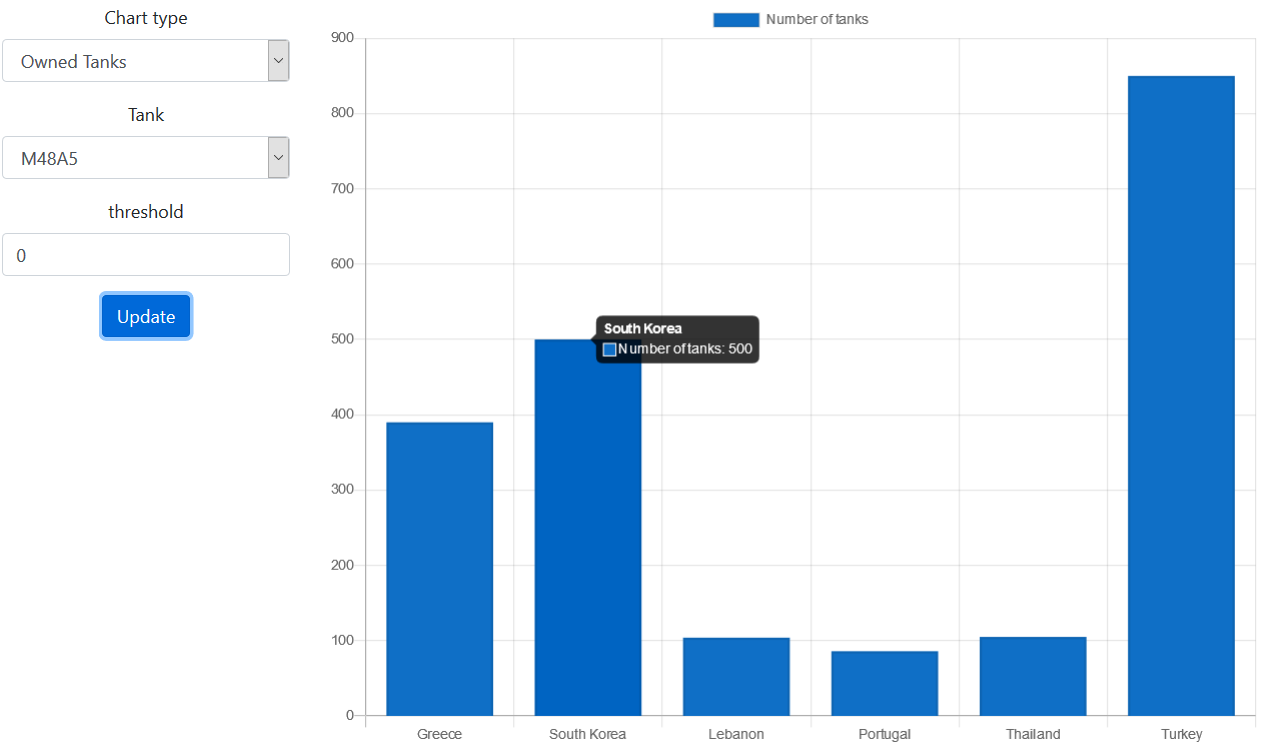
\includegraphics[width=0.9\linewidth]{tex/owned_tanks.PNG}
    \caption{Wykres typu posiadanego uzbrojenia bez ustawionego progu.}
    \label{fig:owned_tanks}
\end{figure}
\begin{figure}[H]
    \centering 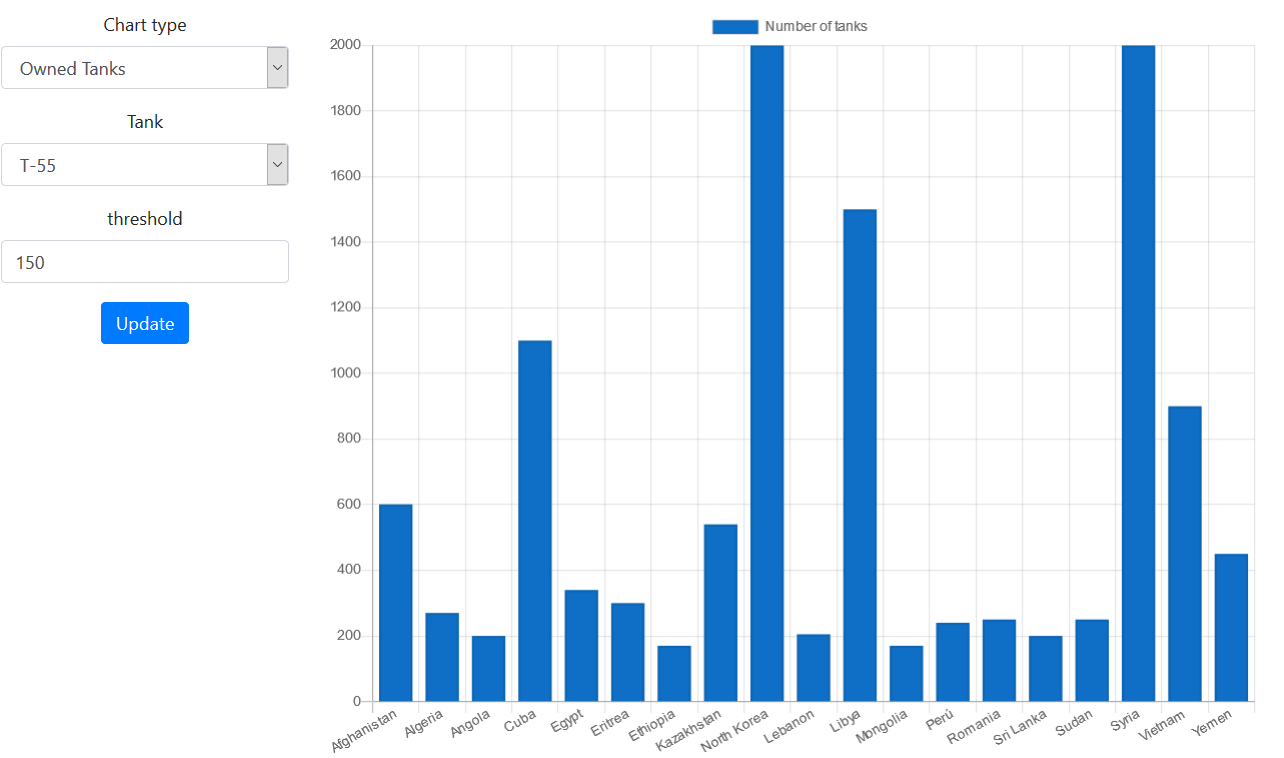
\includegraphics[width=0.8\linewidth]{tex/owned_tanks_treshold.PNG}
    \caption{Wykres typu posiadanego uzbrojenia z ustawionym progiem.}
    \label{fig:owned_tanks_treshold}
\end{figure}
\newpage
\subsection{Graf powiązań}
Kolejnym scenariuszem użycia aplikacji jest stworzenie grafu prezentującego relacje między krajami, w których uzbrojeniu bojowym znajduje się ten sam typ czołgu. Użytkownik będzie mógł określić typ dla którego ma zostać stworzony graf, poprzez wybranie go z listy. Dodatkowo, po zaznaczeniu checkboxu \textit{Alliance Only} jest możliwość zaktualizowania wykresu poprzez zawężenie wyników do państw, będących ze sobą w sojuszach. Ostatnią dostępną opcją jest określenie k-rdzenia dla grafu w celu dalszego ograniczania wyników. 
\begin{figure}[H]
    \centering 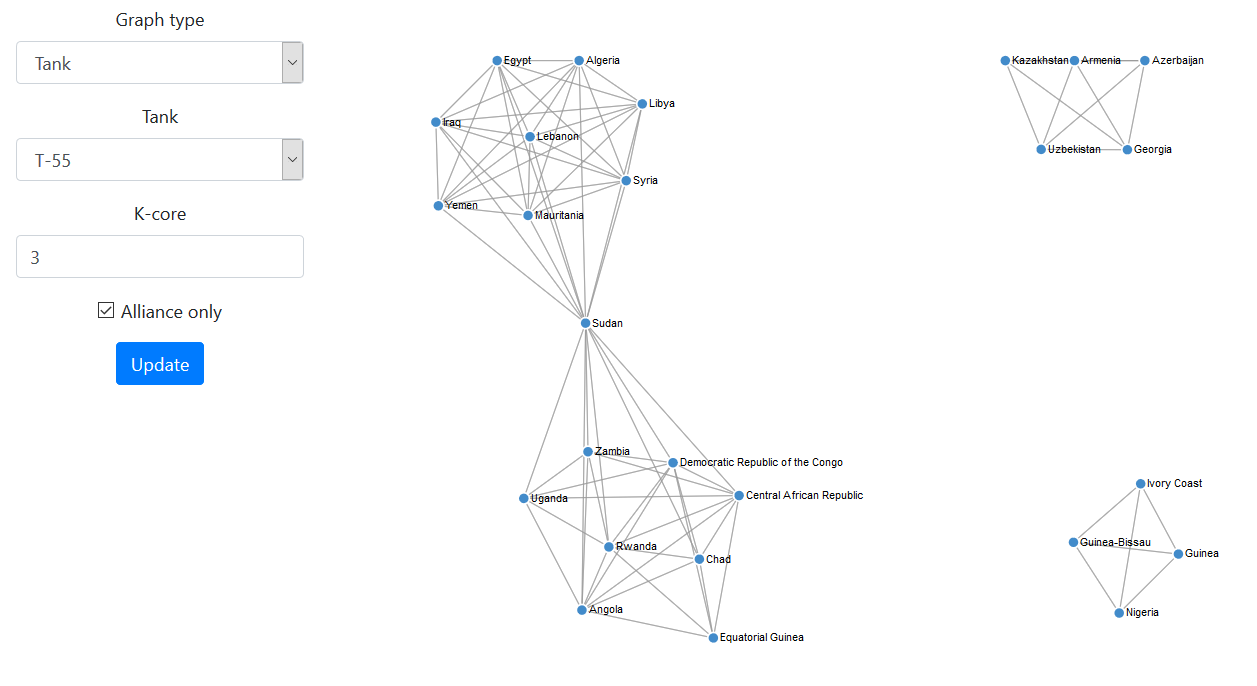
\includegraphics[width=1\linewidth]{tex/tank_graph.PNG}
    \caption{Graf powiązań z ustawioną wartością k-rdzenia.}
    \label{fig:owned_tanks_treshold}
\end{figure}
\subsection{Wykres wielkości produkowanych/posiadanych czołgów}
Ten scenariusz pozwala na stworzenie wykresu słupkowego prezentującego sumaryczną ilość posiadanych czołgów oraz sumaryczną ilość wyprodukowanych przez państwo wozów bojowych. Widok odbiega nieznacznie od tego, który został zaproponowany w koncepcji, która zakładała porównanie sumarycznej ilości wyprodukowanych czołgów oraz sumarycznego eksportu. Obiektywnie oceniając, zaimplementowana opcja prezentuje ciekawszy zbiór wyników. Użytkownik ma możliwość wybrania z listy dowolnej ilości krajów dla których chce przeprowadzić porównanie, a następnie poprzez naciśnięcie przycisku \textit{Update} stworzenie wykresu. Po najechaniu kursorem na dany obszar kolorystyczny wyświetlana jest informacja o kraju, obszarze wykresu (zgodnie z legendą) oraz ilości czołgów. 
\begin{figure}[H]
    \centering 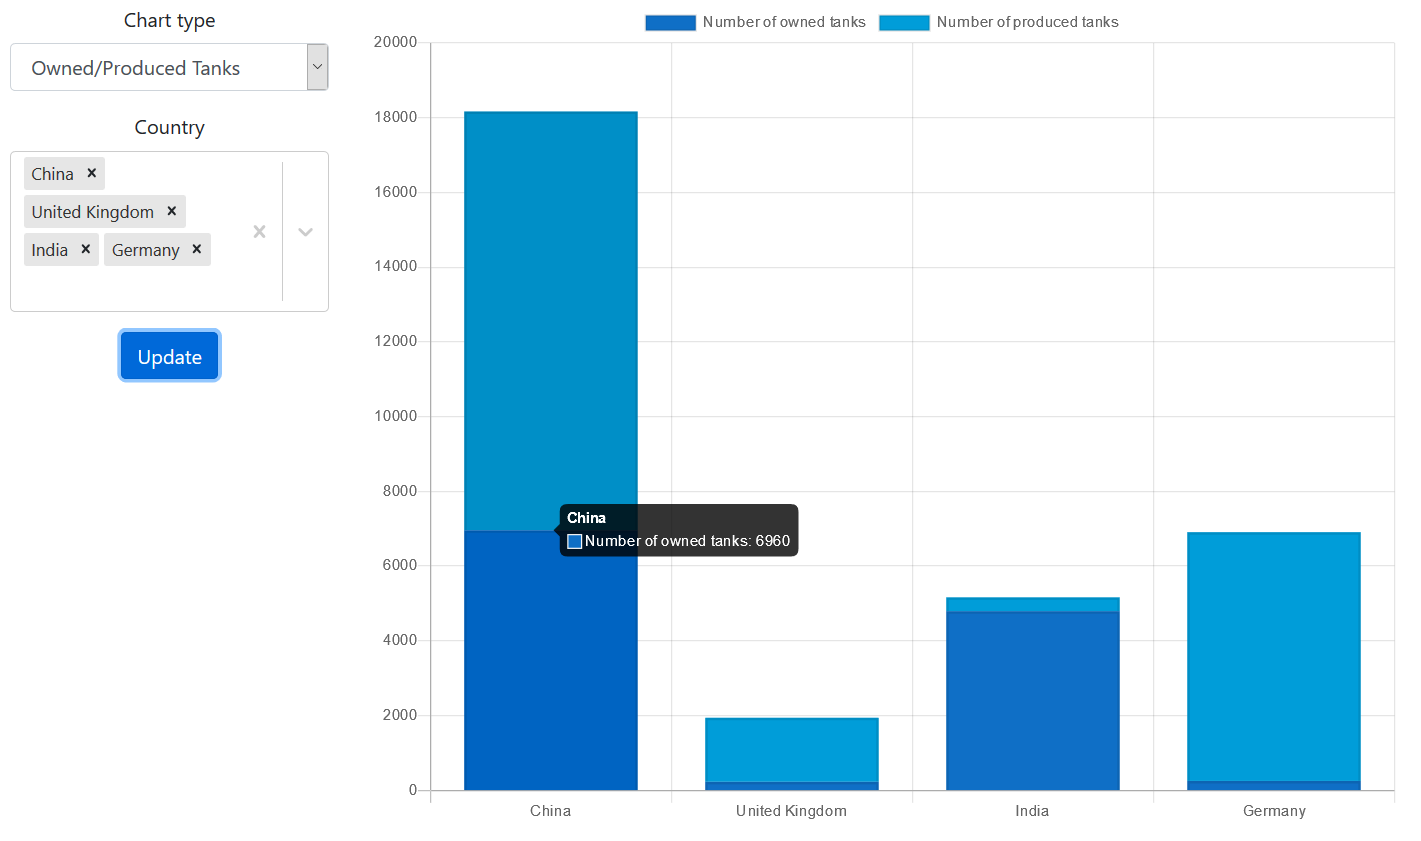
\includegraphics[width=0.9\linewidth]{tex/owned_produced.PNG}
    \caption{Wykres wielkości eksportu}
    \label{fig:owned_exported}
\end{figure}
\subsection{Wykres posiadanych czołgów}
Ten scenariusz użycia aplikacji pozwala na stworzenie wykresu słupkowego prezentującego ilości oraz typy posiadanych czołgów. Użytkownik ma możliwość wybrania z listy interesujących go państw, a następnie, poprzez przyciśnięcie przycisku \textit{Update} stworzenie wykresu porównawczego. Po najechaniu kursorem na dany obszar kolorystyczny pokazuje się informacja o kraju, typie oraz ilości posiadanych czołgów.
\begin{figure}[H]
    \centering 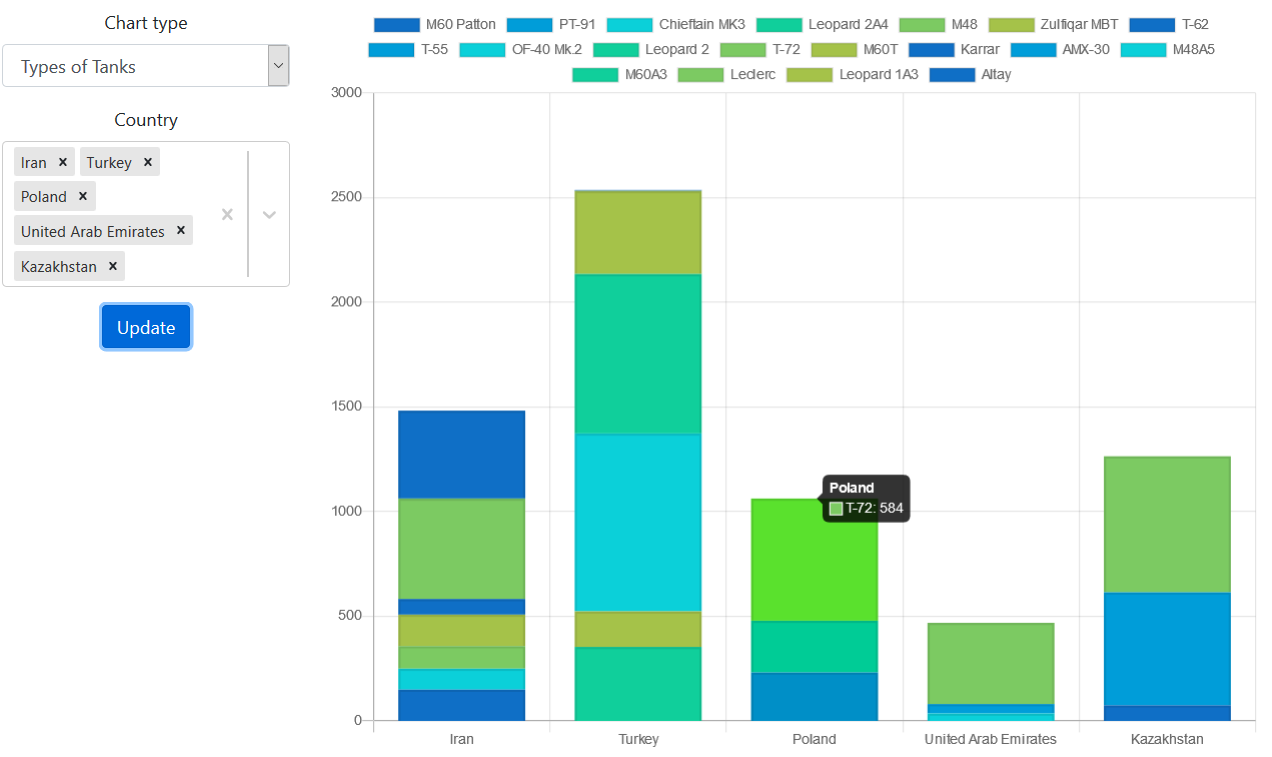
\includegraphics[width=0.9\linewidth]{tex/types_of_tanks.PNG}
    \caption{Wykres posiadanych czołgów.}
    \label{fig:types_tanks}
\end{figure}
\subsection{Graf powiązań}
Jest to graf prezentujący państwa, do których dany kraj eksportował wyprodukowane przez siebie czołgi. Państwo-producent jest zaznaczone kolorem czerwonym. Kolorem zielonym zaznaczone są kraje, które są w sojuszu z wybranym przez użytkownika krajem wytwarzającym czołgi.
\begin{figure}[H]
    \centering 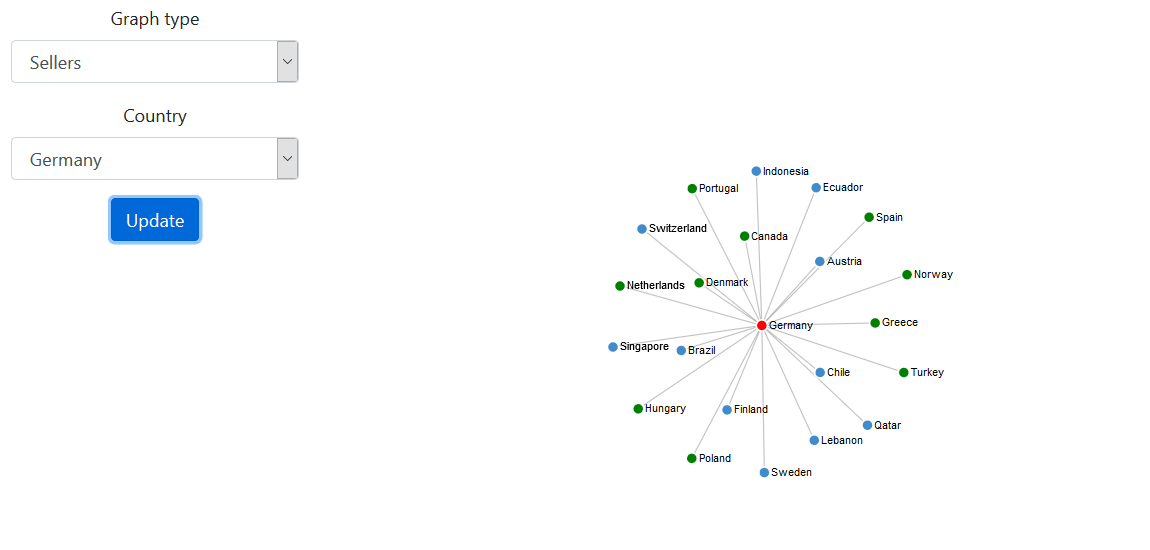
\includegraphics[width=0.8\linewidth]{tex/sellers.PNG}
    \caption{Graf powiązań.}
    \label{fig:sellers_graph}
\end{figure}
\subsection{Graf sojuszy}
Ten scenariusz użycia aplikacji pozwala na wykreślnie grafu sojuszy dla wybranych przez użytkownika państw. Kolorem czerwonym zaznaczone są węzły odpowiadające krajom określonym przez klienta. Krawędziom między państwem wybranym, a jego sojusznikiem zostały nadane unikatowe kolory w celu zwiększenia czytelności wizualizacji. Dodatkowo, po zaznaczeniu checkboxu \textit{K-core} pojawia się możliwość wybrania stopnia rdzenia, który po naciśnięciu przycisku \textit{Update} zostanie przedstawiony na grafie zawężając wyniki. 
\begin{figure}[H]
    \centering 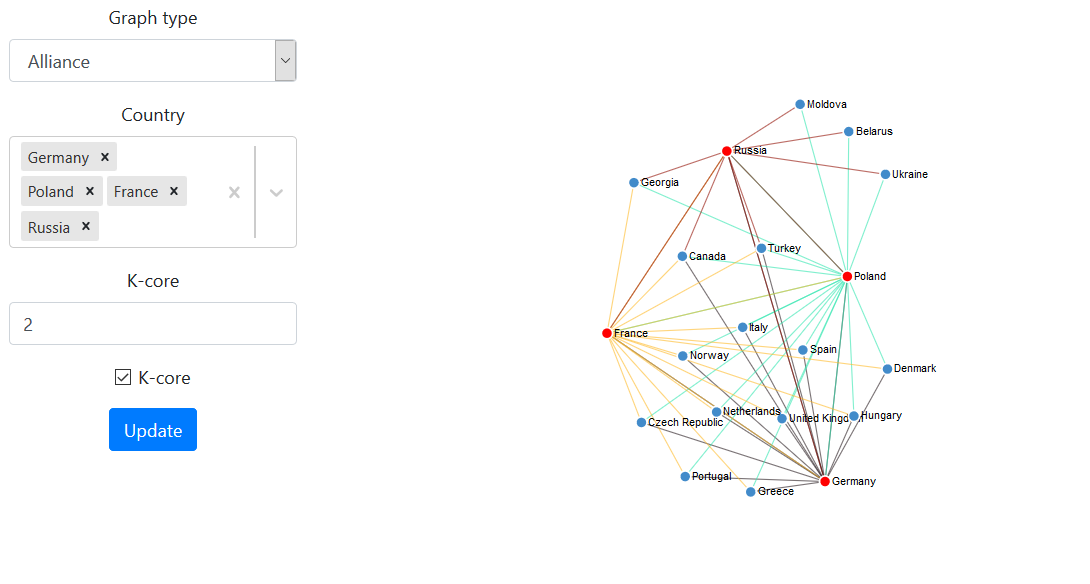
\includegraphics[width=0.8\linewidth]{tex/alliance.PNG}
    \caption{Graf powiązań.}
    \label{fig:alliance_graph}
\end{figure}

\section{Odstępstwa od koncepcji}
Część wykresów posiada niewiele danych - wynika to z różnorodności posiadanego uzbrojenia przez dane państwa.
\\??